\chapter{Implementierung}\label{implementierung}

In diesem Kapitel wird auf Implementierungsdetails des Parsers und die durch ihn erzeugte interne Repräsentation von Formeln eingegangen. Der Unifikationsalgorithmus und das Resolutionsverfahren wurden bereits in Kapitel \ref{konzeption} ausführlich beschrieben. Die Implementierung dieser beiden Algorithmen wird nicht näher beschrieben.

\section{Lexing und Parsing}
Geparst werden Programme aus einer einfachen Textdatei. Im ersten Schritt wird der Eingabetext durch einen regulären Ausdruck in Tokens zerlegt (das sog. lexing). Der reguläre Ausdruck wurde mit der Library cl-ppcre \cite{cl-ppcre} erstellt. Die Syntax für reguläre Ausdrücke in dieser Library entspricht der Syntax von Perl.

\begin{verbatim}
forall|exists|and|<=|=>|:|[a-zA-Z0-9]+\\(.*\\)(?=\\s*<=)
|[a-zA-Z0-9]+\\(.*\\)(?=\\s*and)|[a-zA-Z0-9]+\\(.*\\)(?=\\s*=>)
|[a-zA-Z0-9]+\\(.*\\)(?=\\.)|[a-z]+|\\.
\end{verbatim}

Die ersten sechs Fälle entsprechen vordefinierten Schlüsselwörtern. Die nächsten vier Fälle matchen Prädikatsdefinitionen. Das Ende einer Prädikatsdefinition (die letzte schließende Klammer) wird über einen Lookahead identifiziert. So wird eine Prädikatsdefinition nur dann gematcht, wenn auf sie entweder {\tt <=}, {\tt and}, {\tt =>} oder {\tt .} folgt.

Nachdem der Eingabetext so in Schlüsselwörter und Prädikatsdefinitionen zerlegt wurde, werden für Prädikatsdefinitionen Symbole angelegt und der Name sowie die Argumentenliste in Properties gespeichert. Die Argumentenliste liegt nach diesem Schritt noch als String vor und muss in einem späteren Schritt durch den Termparser geparst werden (Abschnitt \ref{termparser}). Auch für Variablen werden Symbole angelegt, die nach dem Parsen der Terme an den entsprechenden Stellen in die Terme eingefügt werden. So ist sichergestellt, dass die Variablen innerhalb einer Klausel eindeutig, von Klausel zu Klausel jedoch unterschiedlich sind.

\subsection{Parser für Programme}\label{progparser}
Der erste Parser stellt fest, ob die vom Lexer erzeugte Folge von Tokens ein gültiges Programm ist. Es handelt sich dabei um einen $LL(2)$-Parser, da die Eingabe von links nach rechts abgearbeitet wird und anhand eines Lookaheads von zwei Terminalsymbolen eine Ableitung für das am weitesten Links stehende Nichtterminal ausgewählt wird. Geparste Prädikatssymbole werden je nach Position im Programm als positives oder negatives Literal einer Klausel interpretiert und in entsprechenden Properties eines Klauselsymbols gespeichert.

Der Parser ist in mehrere Funktionen aufgeteilt. Gesteuert wird das Parsing in der  Hauptfunktion {\tt parse-program}, die die als nächstes zu expandierenden Nichtterminale, die schon teilweise geparste Tokenfolge sowie die bereits erstellte Klauselmenge verwaltet.

\begin{verbatim}
(defun parse-program (input)
  (do* ((ntl '(s)) ;; Liste der Nichterminale, zu Beginn zur s
       (program input)
       (output NIL)
       (la (take 2 program) 
           (take 2 program)) 
               ;; zwei Terminalsymbole als Lockahead
       (expansion (funcall (next-nt ntl) la) 
                  (funcall (next-nt ntl) la))
               ;; Aufruf der Funktion zum am weitesten 
               ;; links stehenden Nichtterminal
       (production (nth 2 expansion) (nth 2 expansion))
               ;; Zahlencode der gewählten Ableitung
       (to-match (car expansion) (car expansion))
               ;; zu matchende Terminalsymbole
       (new-nt (cadr expansion) (cadr expansion)))
               ;; als nächstes zu expandierende Nichtterminale
    ((and (not program) (not ntl)) (reverse output))
         ;; Abbruchbedingung
    (case production
      ...
      ;; Erweiterung des Output je nach Produktion
      ...
      )
    (setq program (match (car expansion) program))  
            ;; konsumieren der Eingabe von links
    (setq ntl (append new-nt (cdr ntl)))
            ;; erweitern der Nichtterminalliste))
\end{verbatim}

Das expandieren von Nichtterminalen wird anhand eines Lookaheads von gesonderten Funktionen übernommen. Dabei gibt es für jedes Nichtterminal eine Funktion, die anhand des Lookaheads entscheidet, welche Terminalsymbole als nächstes gematcht werden können und welche Nichtterminale als nächstes expandiert werden müssen. Die Regeln nach denen diese Nichtterminalfunktionen arbeiten ergeben sich aus der Grammatik aus Definition \ref{proggramdef}. Wir betrachten hier beispielhaft die Funktion zum Nichtterminal {\tt S}.
\newpage

\begin{verbatim}
(defun s (la)
  (cond ((la-check la '(forall var))
         '((forall) (v k s) 0))
        ((la-check la '(exists var))
         '((exists) (v k s) 1))
        ((la-check la '(lit end))
          '((lit end) (s) 2))
        ((la-check la NIL)
         '(nil nil 3))
        (T (error "no fitting production"))))
\end{verbatim}

Die Funktion erhält aus der Hauptfunktion die nächsten zwei Symbole der Eingabe als Parameter {\tt la}. Die Funktion {\tt la-check} liefert true, falls der Wert der Symbole in {\tt la} den Symbolen im zweiten Argument entsprechen. Diese Funktion ist notwendig, das z. B. die Literaltokens in der Eingabe des Parsers durch den Lexer bereits mit Propertys versehen sind.

Passt der Lookahead zu einer möglichen Produktion wird ein Trippel zurückgeliefert. Das erste Element dieses Trippels ist eine Liste mit Terminalsymbolen, die nun durch die Hauptfunktion gematcht werden können. Die Anzahl der Terminalsymbole ist Situationsbedingt. Ist es anhand des Lookahead möglich mehr als ein oder zwei Terminalsymbole zu matchen so wird dies auch getan.

Das zweite Element des Trippels ist eine Liste mit Nichtterminalen, die als nächstes zu expandieren sind. Diese Liste wird in der Hauptfunktion vorne an die Liste der als nächstes zu expandierenden Nichtterminale angefügt.

Das letzte Element des Trippels ist ein Zahlencode, der die in der Hauptfunktion auszuführenden Aktionen beschreibt. Je nach Antwort der Nichtterminalfunktion werden dann in der Hauptfunktion die nötigen Aktionen angestoßen. Dazu gehören das Anlegen einer neuen Klausel beim Parsen eines Quantors, das Hinzufügen von geparsten Variablensymbolen zur Liste von Variablen einer Klausel oder das setzen eins geparsten Literals als positives oder negatives Literal einer Klausel. So wird bereits beim Parsen eine gewisse Interpretation der Eingabe vorgenommen, die sich in der internen Repräsentation der Daten widerspiegelt.

Die interne Struktur eines geparsten Programms wie sie vom Parser erzeugt wird entspricht der Abbildung \ref{internrep1}

\begin{figure} %[hbtp]
	\centering
		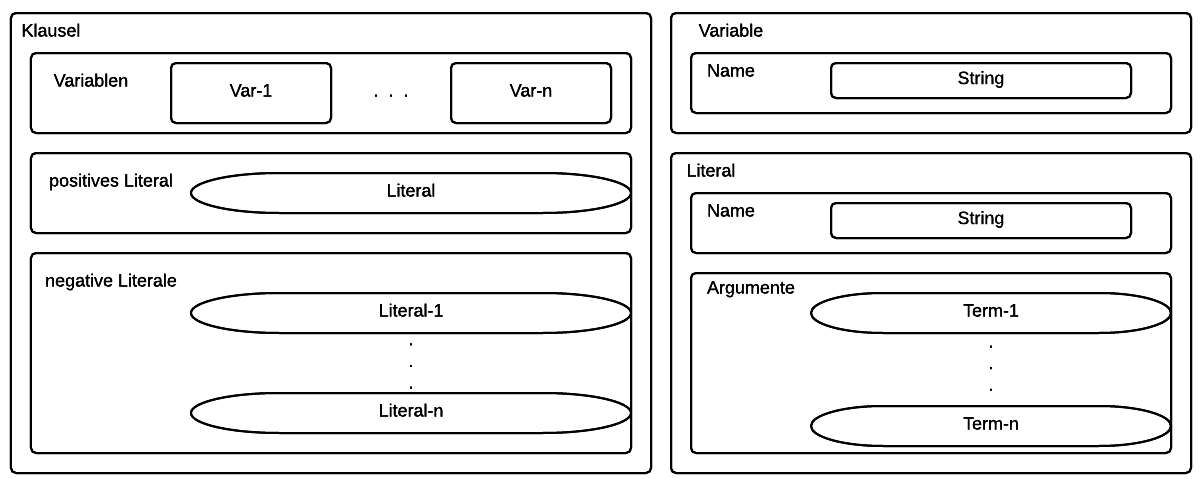
\includegraphics[scale=.7]{/home/steven/dev/lisp/cl-reason/doc/images/internrep1.png}
	\caption{interne Repräsentation von Programmen}
	\label{internrep1}
\end{figure}

\subsection{Parser für Terme}\label{termparser}
Der Parser für Terme wurde durch einen Parsergenerator direkt aus der Grammatik aus Definition \ref{termgram} generiert. Verwendet wurde die Parsergenerator Library cl-yacc \cite{cl-yacc}. Der Erzeugte Parser arbeitet auf einer Folge von Tokens die aus den in Properties der Literale gespeicherten Strings erzeugt werden.
\newpage

\begin{verbatim}
(defun tokenize-terms (termstring)
  (mapcar (lambda (x)
            (cond ((string= x "(") 'LB)
                  ((string= x ")") 'RB)
                  ((string= x "[") 'LS)
                  ((string= x "|") 'CONS)
                  ((string= x "]") 'LE)
                  ((string= x "+") '+)
                  ((string= x "-") '-)
                  ((string= x "*") '*)
                  ((string= x "/") '/)
                  ((string= x ",") 'SEP)
                  ((cl-ppcre:scan "\\d+" x) (parse-integer x))
                  (T (read-from-string x))))
	  (remove " " (all-matches-as-strings *regex-term* termstring) 
                  :test 'string=)))
\end{verbatim}

Auch bei diesem Parser werden nach dem Parsen eines Teils der Eingabe bestimmte Operationen ausgeführt, die die geparsten Terme in eine interne Repräsentation überführen.

\section{Interpreter}
Nachdem ein Großteil der für die Resolution benötigten Informationen bereits durch die Parser in einer geeigneten internen Repräsentation gespeichert wurde, sind nur noch Terme, insbesondere Listen gesondert zu interpretieren.

Da für jede Klausel explizit angegeben werden muss, welche Symbole Variablen sind und für jede Variable bereits durch den Lexer ein Symbol angelegt wurde, müssen lediglich alle Vorkommnisse dieses Symbols in allen Termen einer Klausel durch das bereits existierende Variablensymbol ersetzt werden.

\subsection{Listen}
Der Termparser unterscheidet zwischen konkreten Listen der Form $[t_1,...,t_n]$ und abstrakten Listen der Form $[x|y]$. Für abstrakte Listen kann direkt eine entsprechende Darstellung als Term $cons(x,y)$ abgelesen werden.

Konkrete Listen müssen in einem gesonderten Schritt in diese Form überführt werden. Dazu wird rekursiv aus den geparsten Elementen der Liste ein Funktionsterm erzeugt.

Aus der Liste $[1,2,3,4]$ wird so der Funktionsterm

\begin{equation}
  cons(1,cons(2,cons(3,cons(4,empty))))
\end{equation}

Abbildung \ref{internrep2} zeigt die finale interne Repräsentation von Termen.

\begin{figure} %[hbtp]
	\centering
		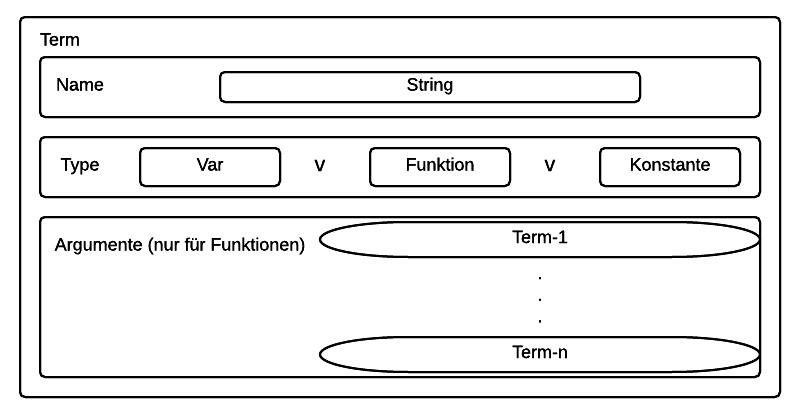
\includegraphics[scale=.9]{/home/steven/dev/lisp/cl-reason/doc/images/internrep2.png}
	\caption{interne Repräsentation von Termen}
	\label{internrep2}
\end{figure}
  
\section{Logisches Schlussfolgern}
Die beiden Kernfunktionen für die Implementierung des Schlussfolgerungssystems sind die Implementierungen des Unifikationsalgorithmus und des SLD-Resolutionsalgorithmus.

Die im Abschnitt \ref{unialg} angegebene rekursive Funktion zur Unifikation von Termlisten wurde rekursiv implementiert. Erweitert auf Literale wird sie während der SLD-Resolution verwendet.

\begin{verbatim}
(defun unify-literals (lit1 lit2) 
  (let ((name1 (get lit1 'name))
        (name2 (get lit2 'name))
        (args1 (mapcar 'copy-term-symbol (get lit1 'args)))
        (args2 (mapcar 'copy-term-symbol (get lit2 'args))))
    (if (and (string= name1 name2)
             (= (length args1)
                (length args2))) 
        (unify-termlists args1 args2 '())
       'fail)))
\end{verbatim}

Da die Anwendung von Substitutionen Teil des Algorithmus ist, ist es nötig, dass während der Unifikation lediglich auf Kopien der Termlisten gearbeitet wird. 

Das im Abschnitt \ref{sld-res} beschriebene Verfahren wurde als iterativer Algorithmus in der Funktion{\tt sld-resolution} implementiert.

Gestartet werden können Programme nach dem Laden des Systems durch einen Aufruf der Funktion {\tt run-program}. Als Argument erhält diese Funktion den Dateipfad des Programms. Da Anfragen direkt mit im Programm stehen, müssen sie durch einen Existenzquantor eingeleitet werden, auch wenn keine Variablen in der Anfrage vorkommen.
